%!TEX root = ../main.tex
\chapter{A Brief Overview of Android Fundamentals}
To understand the reverse engineering process of an Android application, it’s helpful to start with some foundational knowledge. At the most basic level, an Android app is made up of activities and layouts. Activities are special classes, typically written in Kotlin, that control how the app behaves and responds to user input. For example, if an app has a button, the activity defines what happens when that button is clicked. 

Most Android apps have one or more screens, and the design of these screens is handled through layout files or directly in the activity code. Layout files are usually written in XML and can include elements like text, images, and buttons (Head First Android Development). Figure [insert number] shows a diagram of activities and layouts. Figure [insert numbah] illustrates how they interact during actual device use.
\begin{figure}
	\centering
	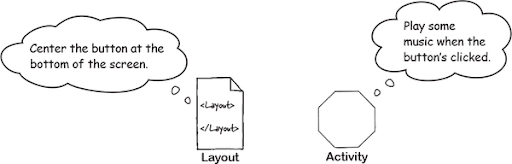
\includegraphics[width=0.7\linewidth]{activity_layout}
	\caption{}
	\label{fig:activitylayout}
\end{figure}
\begin{figure}
	\centering
	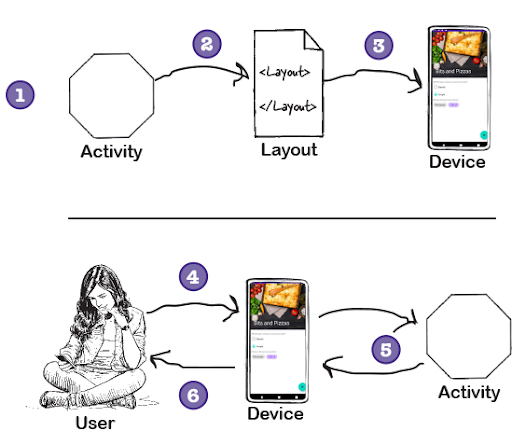
\includegraphics[width=0.7\linewidth]{activity_layout_process}
	\caption{}
	\label{fig:activitylayoutprocess}
\end{figure}

\begin{itemize} 
	\item Android launches the app’s main activity.
	\item The activity instructs Android to use a specific layout.
	\item The layout is displayed on the device.
	\item The user interacts with the layout.
	\item The activity responds to these interactions and updates the display.
	\item The user is able to view the updated display seamlessly.
\end{itemize}

Apps are built using the Android Software Development Kit. The most straightforward place to do this is the Android Studio app. The Android SDK has Android source files and a compiler used to compile code into the Android format.

% TODO: \usepackage{graphicx} required
\begin{figure}
	\centering
	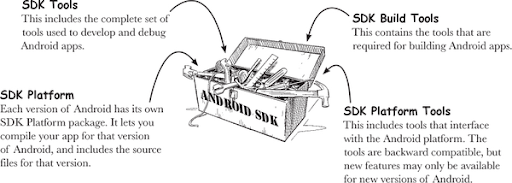
\includegraphics[width=0.7\linewidth]{android_sdk_tools}
	\caption{}
	\label{fig:androidsdktools}
\end{figure}

If you’re familiar with Android, you’ve probably encountered its fun, food-based versioning system. Each Android version includes a version number and a code name. The version number refers to the specific release (like 8.0), while the code name represents a broader release range (like Oreo). Google stopped using dessert-themed code names after Android 9.

Each version of Android also corresponds to an API level, which is used by apps to ensure compatibility. For example, Android 11 corresponds to API level 30.

Android Studio projects use the Gradle build system to compile and deploy apps. Gradle-based projects follow a standard directory structure, which is shown in Figure [insert number here].

% TODO: \usepackage{graphicx} required
\begin{figure}
	\centering
	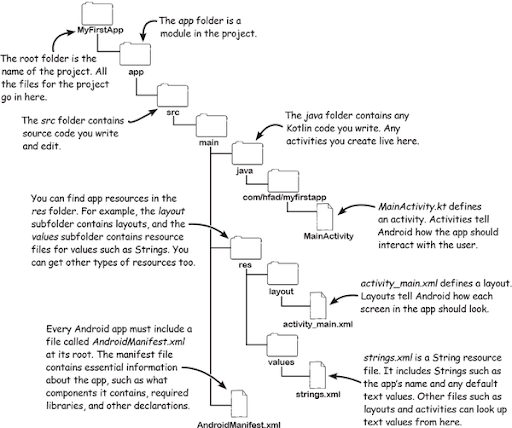
\includegraphics[width=0.7\linewidth]{gradle_build_structure}
	\caption{}
	\label{fig:gradlebuildstructure}
\end{figure}
A much larger version of this structure is seen in the decompilation of the Persolips app. 

An Android app is made up of four main components: activities, services, broadcast receivers, and content providers. Each of these acts as an entry point into the app, either for the user or the system. Some components operate independently, while others rely on or interact with each other.

As mentioned before, Activities are the entry points that users interact with directly. Each activity represents a single screen with a user interface. In a note-taking app, for example, you might have one activity for composing a note, another for creating folders, and another for reading existing notes. While each activity functions independently, they work together to provide a cohesive user experience. Activities can even be started by other apps—if permissions allow. For instance, the Photos app might open a note composition activity so an image can be saved directly into a note.

Activities also manage key interactions between the system and the app. They help Android determine what’s important to the user and ensure that relevant processes are kept running. They track backgrounded processes that might be reopened and help manage killed processes so their state can be restored if needed. Activities enable apps to work together and let the system coordinate those interactions. In code, activities are implemented as subclasses of Android’s Activity class.

Services are also entry points, but they run in the background and are designed for general-purpose tasks rather than direct user interaction. They’re used to keep apps running behind the scenes—for example, to perform long-running operations or interact with remote processes. A service has no user interface. It might do something like keep the flashlight on while a user switches to another app or fetch data from the internet without interrupting the user’s experience. Activities and other components can start services and allow them to run independently or bind to them.

There are two types of services: started services and bound services. A started service continues to run even if the user leaves the app—like keeping the flashlight on or syncing data in the background. Services that the user is aware of (like the flashlight) are handled differently than those that operate silently (like data syncing). Bound services, on the other hand, only run when another component is actively connected to them.

Broadcast receivers allow the system to deliver messages or events to apps, even if the app isn't currently running. This makes it possible to respond to system-wide events outside of the usual user flow. For example, a scheduled notification could be delivered through a broadcast receiver without needing the app to stay open.
Content providers manage access to data stored outside of the app itself, such as in a local SQLite database, on the device, or in the cloud. They make it possible for apps to query or modify this data securely. For example, a social networking app might use a content provider to access the user’s device contacts when adding new friends.

When an Android app is packaged and deployed, it’s bundled into a file called an APK (Android Package Kit). This file contains everything needed to install and run the app on a device. Figure [insert number here] outlines the typical structure of an APK.
Kotlin source code is compiled into bytecode, and libraries and resources are gathered. These elements are then assembled into the APK. The contents of an APK typically include:
\begin{enumerate}
	\item Android launches the app’s main activity.
	\item The activity instructs Android to use a specific layout.
	\item The layout is displayed on the device.
	\item The user interacts with the layout.
	\item The activity responds to these interactions and updates the display.
	\item The user is able to view the updated display seamlessly.
\end{enumerate}

All of these components work together to form the complete, installable app package. When installed, the Android system unpacks the APK and sets up everything the app needs to run on the device.
% TODO: \usepackage{graphicx} required
\begin{figure}
	\centering
	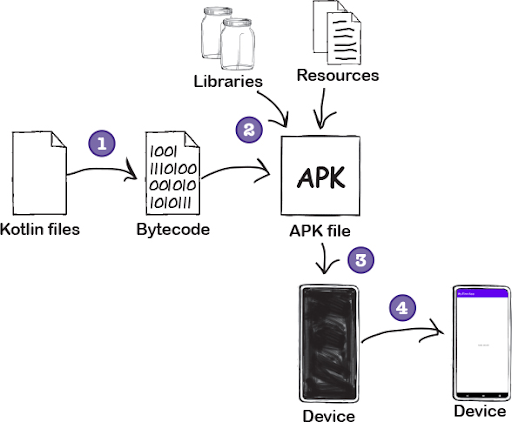
\includegraphics[width=0.7\linewidth]{apk_to_app}
	\caption{}
	\label{fig:apktoapp}
\end{figure}
